\section{Experiment}

\subsection{Participants}
We initially recruited 106 online participants for our user study and evaluation, of which 46 completed the study (30 female). Participants were college students, aged 18 to 25. The reading frequency of news articles among participants ranged from daily to almost never. 

\subsection{Experimental Conditions}
The two conditions in our study were MindMargin and the traditional vertical interface, seeded with 39 existing comments from a news article. We selected a recently published article from the Opinion Section of The Harvard Crimson, titled “Don’t Teach for America.” as seen in figure \ref{fig:crimson}. We chose this article on the basis of its opinionated nature and its relevance both in recent news and to our anticipated participant pool. The article already had over fifty comments, from which we selected the top 39 as ranked by Disqus, the existing commenting system in The Harvard Crimson, to be used in our study. The same comments were used in both conditions. In the traditional vertical interface, they appeared in the identical order as ranked in the original article. In MindMargin, they were anchored to the article based on textual references in the comment.

\begin{figure}
\centering
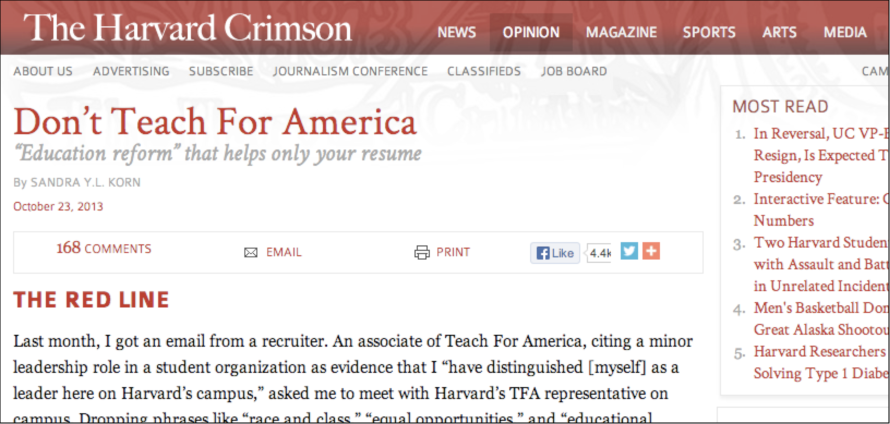
\includegraphics[scale=0.25]{crimson.png}
\caption{The original article from The Harvard Crimson regarding Teach for America (TFA) which was chosen as reference media in our user study.}
\label{fig:crimson}
\end{figure}

\subsection{Design and Setup}
We employed a between-subjects test, with participants assigned randomly to one of the two conditions (19 MindMargin). In order to reproduce the conditions under which one would normally read a news article, we chose to recruit participants online and self-select themselves into reading the article of interest. In order to motivate our participants to actually read or skim the article, instead of skip it, we chose not to use monetary or other time-sensitive incentives. Instead, we chose to design the experiment around the survey question, “Do you (really) think like a Harvard student?”. Figure \ref{fig:landingpage} shows the landing page of our experiment. We then asked participants follow-up questions to verify that they read the article, which included both the overall stance of the article and two pieces of supporting evidence used in the article. Figure \ref{fig:questionnaire} shows the post-experiment questionnaire. Participants were not allowed to refer back to the article once provided the questionnaire. 

\begin{figure}
\centering
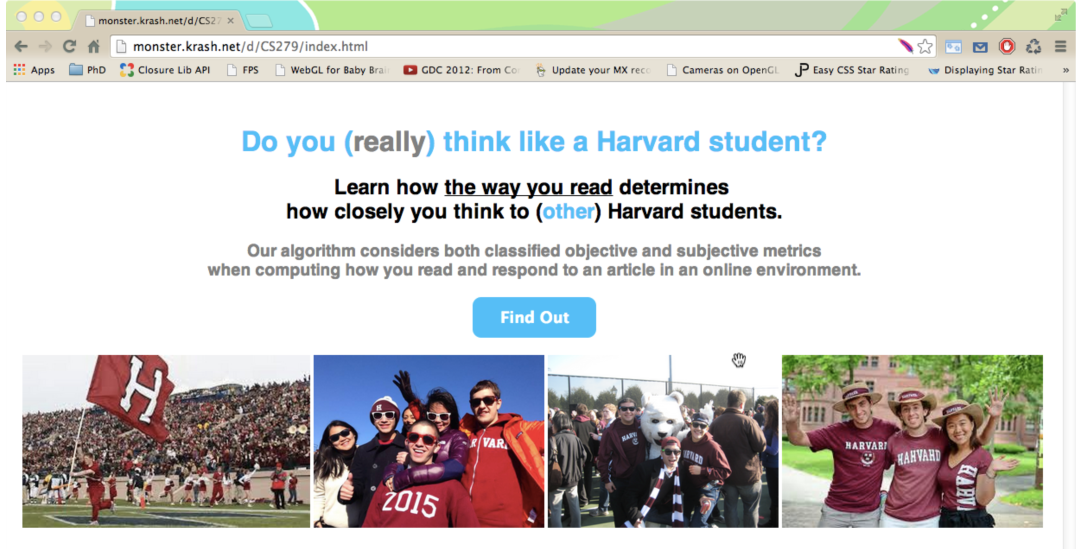
\includegraphics[scale=0.23]{landingpage.png} 
\caption{The landing page of the performed user study.}
\label{fig:landingpage}
\end{figure}

\begin{figure}
\centering
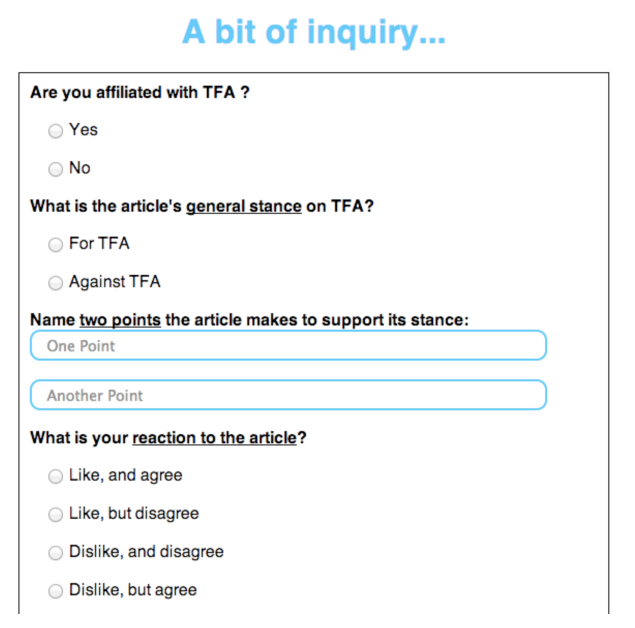
\includegraphics[scale=0.23]{questionnaire.png} 
\caption{Parts of the post-experiment questionnaire.}
\label{fig:questionnaire}
\end{figure}

\subsection{Procedure}
Participants were recruited online through social media and college listservs. They were given an initial questionnaire asking basic demographics and reading frequency. Before given the article, they were also asked to provide a username or pseudonym, or to remain anonymous. During the reading of the article, participants were allotted 10 minutes. After 2 minutes, they were permitted to proceed. The 2-minute delay was to ensure reading of the article, but did not seem to prevent fast readers from proceeding as the average reading time was 3 minutes 47 seconds. In the follow-up questionnaire, reading verification questions were first asked of the article. Participants were also asked their personal stance on the article, whether they liked the article, and whether they agreed with the article. They were also asked to self-report whether they read the comments in the article and to provide two adjectives that described either their reaction to the comments or a description of the comments.
